\documentclass[a4paper,12pt]{article} % добавить leqno в [] для нумерации слева
\usepackage[a4paper,top=1.3cm,bottom=2cm,left=1.5cm,right=1.5cm,marginparwidth=0.75cm]{geometry}

\usepackage[warn]{mathtext}
\usepackage[T2A]{fontenc}
\usepackage[utf8]{inputenc} 
\usepackage[english, russian]{babel}

\usepackage{ upgreek }
\usepackage[table,xcdraw]{xcolor}

\usepackage{indentfirst} %tabutation

\usepackage{amsmath, amsfonts, amssymb, amsthm, mathtools, mathtext} 

\usepackage{graphicx}

\usepackage{wrapfig}
\usepackage{tabularx}

\usepackage{graphicx}%Вставка картинок правильная
\usepackage{float}%"Плавающие" картинки
\usepackage{wrapfig}% Обтекание фигур (таблиц, картинок и прочего)

%%% Дополнительная работа с математикой
\usepackage{amsmath,amsfonts,amssymb,amsthm,mathtools} % AMS





%%% Заголовок
\author{Устюжанина Мария Алексеевна}
\title{Лабораторная работа №1.6.1

Изучение физического маятника
}
\date{\today}

\begin{document}

\begin{titlepage}
	\begin{center}
		{\large МОСКОВСКИЙ ФИЗИКО-ТЕХНИЧЕСКИЙ ИНСТИТУТ (НАЦИОНАЛЬНЫЙ ИССЛЕДОВАТЕЛЬСКИЙ УНИВЕРСИТЕТ)}
	\end{center}
	\begin{center}
		{\large Физтех-школа радиотехники и кибернетики.}
	\end{center}
	
	
	\vspace{4.5cm}
	{\huge
		\begin{center}
			{\bf Отчёт о выполнении лабораторной работы 1.4.1}\\
			 Изучение физического маятника.
		\end{center}
	}
	\vspace{2cm}
	\begin{flushright}
		{\LARGE Автор:\\ Устюжанина Мария Алексеевна \\
			\vspace{0.2cm}
			Б01-107}
	\end{flushright}
	\vspace{8cm}
	\begin{center}
		Долгопрудный 2021
	\end{center}
\end{titlepage}

\section*{Введение}

\begin{wrapfigure}[17]{r}{0.17\linewidth} 
\vspace{-5ex}
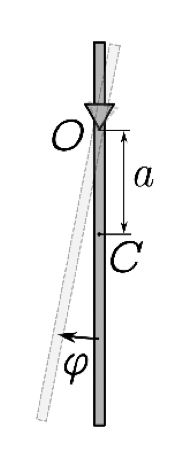
\includegraphics[width=\linewidth]{Маятник1}
\caption{Стержень как физический маятник}
\label{fig:somelabel}
\end{wrapfigure}
\medskip
\textbf{Цель работы:}
\begin{enumerate}
	\item на примере измерения периода свободных колебаний физического маятника познакомиться с систематическими и случайными погрешностями, прямыми и косвенными измерениями;
	\item проверить справедливость формулы для периода колебаний физического маятника и определить значение ускорения свободного падения;
	\item убедиться в справедливости теоремы Гюйгенса об обратимости точек опоры и центра качания маятника;
	\item оценить погрешность прямых и косвенных измерений и конечного результата.
\end{enumerate}

\medskip

\textbf{В работе используются:} металлический стержень с опорной призмой; закреплённая на стене консоль; подставка с острой гранью для определения цента масс маятника; секундомер; линейки металлические различной длины; электронные весы.
\medskip




\textbf{Теоритические сведения}

\begin{wrapfigure}[17]{r}{0.2\linewidth} 
\vspace{-5ex}
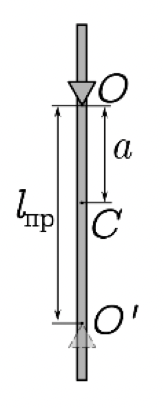
\includegraphics[width=\linewidth]{Маятник2}
\caption{К теореме Гюйгенса}
\label{fig:somelabel}
\end{wrapfigure}

Физический маятник - твёрдое тело, спoсобное совершать колебания в вертикальной плоскости, при подвешивании за одну из точек в поле тяжести.

В данной работе в качестве физического маятника используется однородный стальной стержень длинной 1 метр (L). На стержне закреплена опорная призма, острое ребро которой является осью качания маятника. Призму можно перемещать вдоль стержня, меняя таким образом расстаяние от точки опоры маятника до его центра масс.


\textit{Закон движения твердого тела} для материальной точки, вращающейся на расстоянии r от оси:

\[ M = J\frac{d\omega}{dt};\]

в котором $M=Fr$ - момент силы, относительно оси вращения;
$ J= mr^2$ - момент инерции точечного тела;
$\omega$ - угловая скорость вращения.

Закон вращательного движения для твердого тела, состоящего из совокупности материальных точек:

\[ J = \sum\limits_{i}m_ir^2_i;\]
где $r_i$ - расстояние от точки массой$m_i$ до оси вращения.

Момент инерции стержня, подвешанного на расстоянии $a$ от центра масс, по теореме Гюйгенса-Штейнера определяется:
\[J=\frac{ml^2}{12}+ma^2\]

Период колебаний произвольного физического маятника:
\[ T= 2\pi \sqrt{\frac{J}{mga}}=2\pi \sqrt{\frac{\frac{l^2}{12}+ a^2}{a \cdot g }}; \]
где $l$ - длина стержня, $a$ - расстояние от оcи вращения до центра масс.

Учитывая влияние подвесной призмы, можно найти ускорение свободного падения:
\[T == 2 \pi \sqrt{\frac{J_{стер}-J_{призм}}{m_{стер}ga_{стер}-m_{призм}ga_{призм}}}= 2\pi \sqrt{\frac{\frac{l^2}{12}+a^2}{g(1+\frac{m_{призм}}{m_{стер}})x_{c}}};\]

где $x_c=\frac{m_{стер}a_{стер}-m_{призм}m_{призм}}{m_{стер}+m_{призм}}$- расстояние от центра масс системы до точки подвеса.

Пусть $1+\frac{m_{призм}}{m_{стер}} = \beta$, тогда:

\[ T= 2\pi \sqrt{\frac{\frac{l^2}{12}+a^2}{g\cdot \beta \cdot x_c}}\]

\[ g = \frac{4\pi ^ 2(\frac{l^2}{12}+a^2)}{T^2 \cdot \beta \cdot x_c}\]

 

\newpage
\section*{Результаты измерений и обработка данных}

\begin{enumerate}
\item Абсолютная погрешность линейки $\sigma_{лин}=0,5$мм и секундомера $\sigma_{сек}=0,01$c.

\item Длина стержня $l=(1000,0 \pm 0,5)$мм.

Масса призмы $m_{призмы}= (74,0 \pm0,5)$г.

Масса штанги $m_{штанги} = (1022,5 \pm 0,5)$г.

$\beta = 1 + \frac{m_{пр}}{m_{ст}}\approx 1,07$

\item Положение острия призмы относительно ц.м. стержня в первом эксперименте: $a=(250\pm0,5)$мм.
Положение ц.м. относительно острия призмы $x_{ц.м.} = (235,0\pm 0,5)$мм.
\item Предварительный опыт по измерению периода колебаний:

Количество колебаний: $n=10$;

Время: $t = (15,42 \pm 0,01)$c;

Период колебаний $T=\frac{t}{n}=1,54$c.

Вычислим значение предварительное $g$ по одному измерению:
\[g=\frac{4\pi^2(\frac{l^2}{12}+a^2)}{T^2\cdot \beta \cdot x_ц}= \frac{4\cdot3,14^2(\frac{1^2}{12}+0,25^2)}{1,54^2 \cdot 1,07 \cdot 0,235} \approx9,62  м/c^2\]
Полученное значение для ускорения свободного падения отличается не более, чем на 10\% от табличного.

\item Для определения случайной погрешности измерения времени с помощью секундомера проведем 10 измерений. Результат этого эксперимента занесем в таблицу:

    \begin{tabular}{l|llllllllll}
    № опыта & 1     & 2     & 3     & 4     & 5     & 6     & 7     & 8     & 9     & 10    \\ \hline
    t, сек  & 15,42 & 15,25 & 15,38 & 15,49 & 15,19 & 15,44 & 15,34 & 15,37 & 15,21 & 15,29 \\
    \end{tabular}

\item Среднее значение полученных : $\underline{t} = 15,42$c;

Случайная погрешность: $\sigma^{случ}_t=\sqrt{\frac{1}{N-1} \sum(t_i-\overline{t})^2} \approx 0,1c$;

Систематическая погрешность секундомера: $\sigma^{сист}_{t}\approx 0,01c$;

Полная погрешность: $\sigma^{полн}_{t}\approx 0,1c$.
\item Оценим число колебаний n, по которому следует измерять в период, чтобы относительная погрешность измерения периода соответствовала точности измерений $\mathcal{E} = 0,1\%$:

 Погрешность периода $\sigma_T = \frac{\sigma_t}{n}\approx 0,01c$;

 Относительная погрешность: $\mathcal{E}_t=\frac{\sigma_T}{T}\approx 0,0066$;

 Необходимое число колебаний: $n=\frac{\sigma_T}{T\cdot \mathcal{E}_T}\approx 10$.

\item Проведем опыты для 10 разных значений $a$ и рассчитаем ускорение свободного падения. Результат вычислений:

    \begin{tabular}{l|l|l|l|l|l|l}
    № опыта & a, мм & x, мм & n  & t, сек & T, сек & g, $м/с^2$ \\ \hline
    1       & 50    & 45    & 10 & 26,31  & 2,63   & 10,17         \\ \hline
    2       & 120   & 110   & 10 & 18,09  & 1,81   & 10,2          \\ \hline
    3       & 220   & 205   & 10 & 15,62  & 1,56   & 9,72          \\ \hline
    4       & 300   & 280   & 10 & 15,16  & 1,52   & 9.94          \\ \hline
    5       & 460   & 430   & 10 & 16,13  & 1,61   & 9,73          \\ \hline
    6       & 350   & 315   & 10 & 15,6   & 1,56   & 9,91          \\ \hline
    7       & 250   & 235   & 10 & 15,34  & 1,53   & 9,73          \\ \hline
    8       & 180   & 168   & 10 & 16,34  & 1,63   & 9,57          \\ \hline
    9       & 100   & 92    & 10 & 19,53  & 1,95   & 9,81          \\ \hline
    10      & 30    & 28    & 10 & 33,91  & 3,39   & 9,65          \\
    \end{tabular}


\item Определим приведенную длину маятника:

а) $l_{пр}=a+\frac{l^2}{12\cdot a}=0,25+\frac{1^2}{12\cdot 0,25}\approx 0,583м$;

б) Для физического маятника: $T = 1,53c$

Для математического: $T=2\pi\sqrt{\frac{l_{пр}}{g}}= 2\cdot 3,14 \cdot \sqrt{\frac{0,583}{9,8}}\approx 1,5c$;

в) Проверим справедливость теоремы Гюйгенса: поместим призму в центр качания и перевернем маятник; измерим период $T=1,6c$. Период колебаний в пределе погрешности опыта, следовательно, теорема справедлива.



\item Cреднее значение для ускорения свободного падения:
\[\overline{g}\approx 9,83 м/с^2\]
\[\sigma_g = \sqrt{\frac{1}{N-1}\sum{(g_i-\overline{g})}}\approx 0,18 м/с^2\]
\item График зависимости периода колебаний T от расстояния подвеса a:
\begin{figure}[h]
\centering
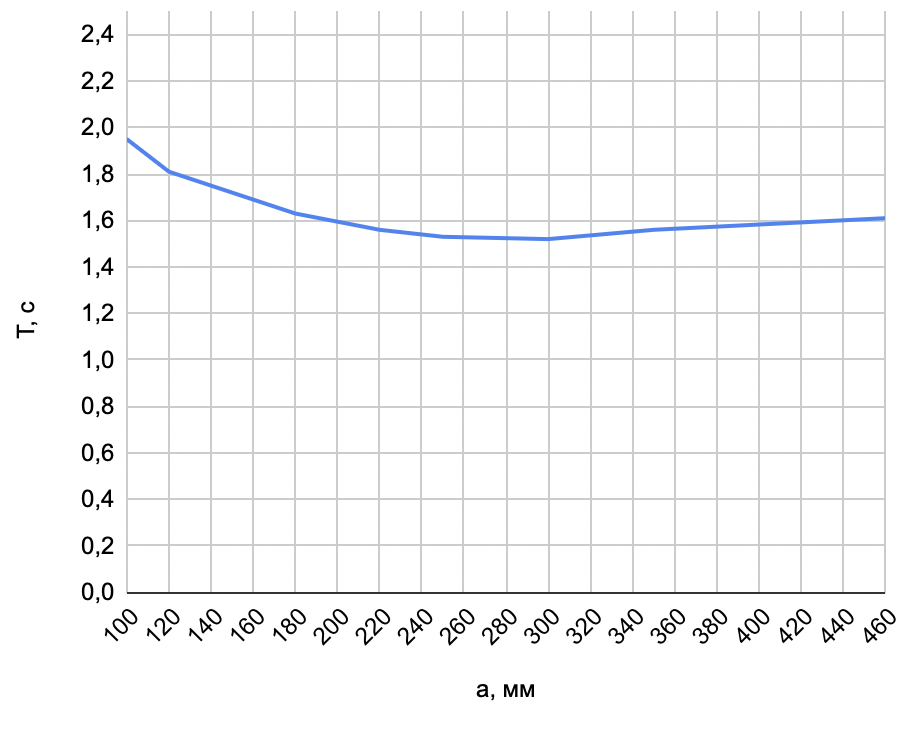
\includegraphics[width=0.6\linewidth]{График}
\label{fig:mpr}
\end{figure}

\item Построим график, откладывая по оси абсцисс величину $U= T^2\cdot x_ц$, а по оси ординат величину $V=a^2$

\begin{figure}[h]
\centering
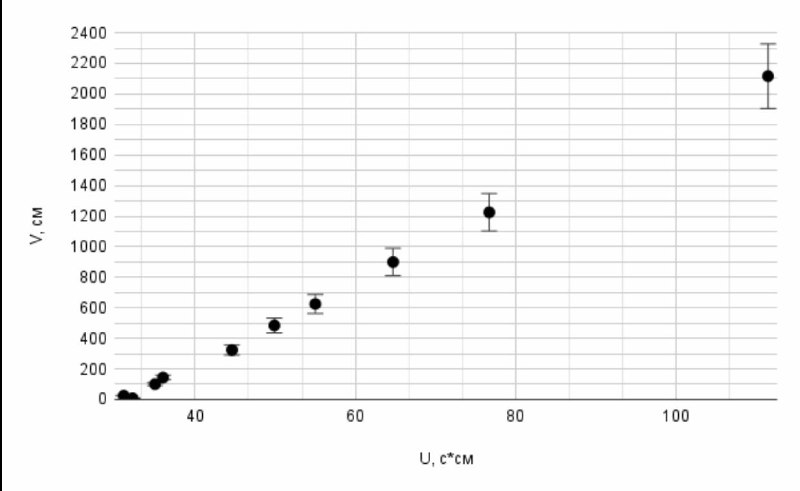
\includegraphics[width=0.6\linewidth]{График2}
\label{fig:mpr}
\end{figure}

\newpage
\item С помощью метода наименьших квадратов определим параметры $k, b$ наилучшей прямой $V=b+kU$ и их погрешность $\sigma_k$, $\sigma_b$:

\[T = 2 \pi \sqrt{\frac{\frac{l^2}{12}+a^2}{g\beta x_{ц}}}\]

\[a^2 = \frac{T^2g\beta x_{ц}}{4\pi^2}-\frac{l^2}{12}\]

\[V = \frac{g\beta U}{4\pi^2}-\frac{l^2}{12}=kU+\beta\]

Следовательно, 
\[k=\frac{g\beta}{4\pi^2}\]
\[g=\frac{4\pi^2k}{\beta}\]

По графику найдем значения k:

\[k=\frac{<UV>-<U>\cdot<V>}{<U^2>\cdot<U>^2}\approx 26,46 см/с^2 \approx 0,26 м/с^2\]

\[\sigma_k=\frac{1}{\sqrt{10}}\cdot \sqrt{\frac{<UV>-<U>\cdot<V>}{<U^2>\cdot<U>^2}-k^2}\approx 0,053м/с^2\]

Найдем ускорение свободного падения: 

\[ g \approx 9,75 м/с^2\]

\[\sigma_g = g\cdot \frac{\sigma_k}{k}\approx 0,19 м/с^2\]

Итак, 

\[g\approx (9,75\pm0,19)м/с^2\]


\end{enumerate}



\subsection*{Вывод}

При помощи усреднения значений ускорения свободного
 падения получили результат с погрешностью около 1,8\%.

 При вычислении через наименьшие квадраты - около 1,9\%.

 Данные получены с примерно равной точностью, и ответ близок к табличному.

 Также в ходе работы была проверена т. Гюйгенса-Штейнера об обратимости точек опоры и центра качания маятника.

\end{document}

